\newif\ifml
\mltrue
%\longtrue

\newif\ifita
%\itatrue
\itafalse

\ifita
\newcommand{\itascore}[1]{\textcolor{red}{(GII-GRIN-SCIE Rating: #1)}}
\else
\newcommand{\itascore}[1]{}
\fi

\documentclass[margin, 10pt]{article} % Use the res.cls style, the font size can be changed to 11pt or 12pt here

\usepackage{xcolor}
\usepackage{graphicx}
\usepackage{hyperref,url}
\usepackage[utf8]{inputenc}
\usepackage{graphicx}

\usepackage{hyperref}
\hypersetup{
    colorlinks=true,
    linkcolor=blue,
    filecolor=magenta,      
    urlcolor=blue,
    pdftitle={Overleaf Example},
    pdfpagemode=FullScreen,
    citecolor = blue,
    }
 \usepackage{adjustbox}
 
 

\usepackage{titlesec}

\usepackage{helvet} % Default font is the helvetica postscript font
%\usepackage{newcent} % To change the default font to the new century schoolbook postscript font uncomment this line and comment the one above

\setlength{\textwidth}{5.in} % Text width of the document

\titleformat{name=\section,numberless}
  {\normalfont\large\bfseries}{}{-1cm}{}
  
 \usepackage[vmargin={1cm,1cm}, hmargin={2cm}]{geometry}

\begin{document}
\pagestyle{empty}



%----------------------------------------------------------------------------------------
%	NAME AND ADDRESS SECTION
%----------------------------------------------------------------------------------------
\moveleft-1.5\hoffset\centerline{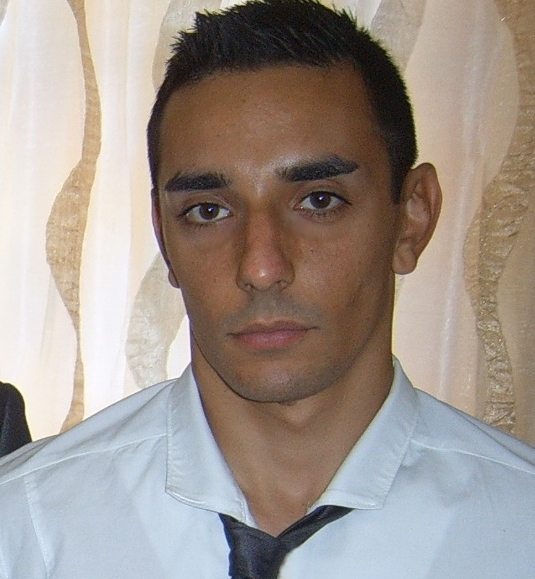
\includegraphics[scale=0.035]{me/me}}
\moveleft.5\hoffset\centerline{\large\bf Dario Pasquini, Ph.D.} % Your name at the top
\moveleft.5\hoffset\centerline{19/09/1991, Rome, Italy.} % Your name at the top
%\moveleft.5\hoffset\centerline{pasquini.dario.1991@gmail.com} 


%\vspace{-5cm}
 %\moveleft.5\hoffset\centerline{pasquini.dario.1991@gmail.com} 
 %\moveleft.5\hoffset\centerline{\textbf{Personal page:} \url{https://pasquini-dario.github.io/me/}}
 %\moveleft.5\hoffset\centerline{\textbf{GitHub:} \url{https://github.com/pasquini-dario/}}
 \vspace{.4cm}
 \moveleft.5\hoffset\centerline{
 \href{mailto:pasquini.dario.1991@gmail.com}{Contact} \qquad
 \href{https://pasquini-dario.github.io/me/}{Personal Page} \qquad
\href{https://github.com/pasquini-dario/}{GitHub} \qquad
  \href{https://scholar.google.com/citations?user=L38xA_8AAAAJ&hl}{Google Scholar}
  }
  

 
\moveleft\hoffset\vbox{\hrule width\textwidth height 1pt}\smallskip % Horizontal line after name; adjust line thickness by changing the '1pt'
 



%----------------------------------------------------------------------------------------


%----------------------------------------------------------------------------------------
%	OBJECTIVE SECTION
%----------------------------------------------------------------------------------------
 
%\section*{Bio:}  
\vspace{.2cm}
 %\noindent Machine Learning Researcher operating at the bleeding edge of the intersection of Security and ``AI'', seeking security and privacy for intelligent systems that transcend trust, ideal assumptions, and optimistic threat models \textcolor{gray}{(\textit{although, in practice, I end up spending most of my day either breaking ML models or building ML models to break stuff})}.
 \ifita
 \noindent Researcher working on the intersection of Security and ``AI'', seeking security and privacy solutions that transcend trust, ideal assumptions, and optimistic threat models. Applying Machine Learning techniques to cybersecurity challenges.
 \else
  \noindent Working on the intersection of Security and ``AI'', seeking security and privacy solutions that transcend trust, ideal assumptions, and optimistic threat models \textcolor{gray}{(\textit{although, in practice, I end up spending most of my day either breaking ML models or building ML models to break stuff})}.
 \fi
 % \noindent \textit{Security} researcher seeking security and privacy solutions that transcend trust, ideal assumptions, and optimistic threat models \textcolor{gray}{(\textit{although, in practice, I end up spending most of my day either breaking ML models or building ML models to break stuff})}.
 

\subsection*{Working on:} 
\itemsep0em 
\begin{itemize}
\itemsep0em 
\item Security \& Privacy in Machine Learning:
	\begin{itemize}
	\item[$\bullet$] Large Language Models \cite{nes, llmmap, hackai}
		\item[$\bullet$]  Private Collaborative Learning \cite{dl, CCS21, CCS22}  		
	\end{itemize}
\item Password Security (using ML) \cite{uncm, SP21, adam}
\item (Attacking and Patching) Cryptosystems (using ML) \cite{MIGP, CCS22} 
\item Differential Privacy \cite{uncm}
\item \textcolor{gray}{[inactive]
 HPC; GPGPU, Multi-GPU \cite{MONOAMG}}
\end{itemize}

\noindent\makebox[\linewidth]{\rule{.8\paperwidth}{0.3pt}}


\section*{Work experience:} 

\begin{description}
	
\item[[ {11/2024 - Now}]] \textbf{Principal Researcher} (\textit{AI \& Security)}\textbf{:}\\
 \textbf{\textit{RSA Conference}}\\
 \textit{Switzerland}

\item[[ {04/2024 - 10/2024}]] \textbf{Visiting Faculty:}\\
%\textbf{where:}
 \textbf{\textit{George Mason University}},  \textit{Cybersecurity department}\\
 \textit{Virginia, USA}
%\textbf{what:} \textit{``Leading research on Large Language Models manipulation and privacy implications.''}

\item[[ {10/2021 - 03/2024}]] \textbf{Postdoctoral Researcher:}\\
%Swiss Federal Institute of Technology Lausanne (EPFL), Switzerland\\
%\textbf{where:} 
 \textbf{\textit{École Polytechnique Fédérale de Lausanne (EPFL)}}\\ 
Security and Privacy Engineering Laboratory (SPRING)\\
\textit{Switzerland}
%\textbf{what:} \textit{``Leading research on: (1)~Security and Privacy of Machine Learning: Private Collaborative Learning and Large Language Models. (2)~Leading research on Machine Learning applications to security: Password Security and Cryptosystems.''}
%Referent: \textit{Prof. Carmela Troncoso }(\textit{carmela.troncoso@epfl.ch})
\item[[ 05/2020 - 9/2021]] \textbf{Research Fellow:}\\
%\textbf{where:} 
 \textbf{\textit{National Research Council (CNR)}}, 
Institute for applied mathematics ``Mauro Picone'' (IAC)\\
\textit{Italy}
%\textbf{what:} \textit{``Research and development of high performance, distributed, Multi-GPUs, solver for massive systems of linear equations.}''
%Research and deployment of Multi-GPUs 
%Referent: \textit{Prof. Massimo Bernaschi} (\textit{massimo.bernaschi@cnr.it})
%\item[[ 2017 -  today]] \textbf{Collaborator IAC-CNR:}\\
%Institute for applied mathematics "Mauro Picone" (IAC), Rome, Italy
\item[[ 04/2019 - 04/2020]] \textbf{Visiting Researcher}:\\
%\textbf{where:} 
 \textbf{\textit{Stevens Institute of Technology}}, \textit{Computer Science department}\\ 
\textit{New Jersey, USA}
%\textbf{what:} \textit{``Leading research on (1)~applications of Deep Learning in Password Security (2)~ Adversarial Machine Learning.}''
%	Host: \textit{Prof. Giuseppe Ateniese} (\textit{ateniese@gmu.edu})
	
%\noindent\makebox[\linewidth]{\rule{.1\paperwidth}{0.3pt}}
\section*{\normalsize{Contract \& Consulting work:}}
\vspace{-.35cm}
\begin{description}
	\item[[ 12/2023]] \textbf{Password Recovery Expert} (Cryptocurrency)\\
	 DSEC Labs LLC, Virginia, USA
	 \item[[ 04/2024]] \textbf{Machine Learning Expert} (Security Auditing of Authentication Systems)\\
	Detack GmbH, Germany\\
	
\end{description}
\end{description}
\noindent\makebox[\linewidth]{\rule{.2\paperwidth}{0.3pt}}


\section*{Education:} 

\begin{description}
\item[[ 2018 - 2021]] \textbf{\textit{Ph.D.}  in  Computer Science} (fellowship winner):\\
\textit{Sapienza} University of Rome, Italy\\
Advisor: \textit{Prof. Massimo Bernaschi} (\textit{massimo.bernaschi@cnr.it})\\


\item[[ 2015 - 2017]] \textbf{Master degree} in  \textbf{Computer Science}: \\
\textit{Sapienza} University of Rome, Italy\\
Final Grade: \textit{110/110} \textit{cum laude}\\
Program of Study: \textit{Network and Security}
%Thesis subject: \textit{Adversarial Neural Cryptography}

\end{description}


\noindent\makebox[\linewidth]{\rule{.2\paperwidth}{0.3pt}}


\ifita
\section*{Technical Skills  \small{\textcolor{gray}{(at least, the ones you might want to pay me for)}}:}
\else
\section*{Technical Skills:}
\fi 
\begin{itemize}
	\item  \textbf{Machine Learning:} 
	\begin{itemize}
		\item TensorFlow (e.g., \href{https://github.com/TheAdamProject/UniversalNeuralCrackingMachines}{UniversalNeuralCrackingMachines}, \href{https://github.com/TheAdamProject/adams}{ADAMS}, \href{https://github.com/pasquini-dario/SplitNN_FSHA}{SplitNN\_FSHA}, \href{https://github.com/pasquini-dario/PLR}{PLR})
		\item PyTorch (e.g., \href{https://github.com/pasquini-dario/LLM_NeuralExec}{LLM\_NeuralExec})
	\end{itemize}
	
	\textbf{General purpose languages \& libs}:
	\begin{itemize}
		\item Python
		\item MPI, CUDA (e.g., \href{https://github.com/bootcmatch/BootCMatchG/}{BootCMatchG})
		\item  C / C++
	\end{itemize}
	
\end{itemize}

\noindent\makebox[\linewidth]{\rule{.2\paperwidth}{0.3pt}}
\section*{Academic service:}  
\begin{itemize}
	\item \textbf{Program committees:}
	\begin{itemize}
		\item ACM CCS 2023
		\item USENIX Sec. 2023, 2025
		\item IEEE SaTML 2024, 2025
		\item PETS 2025.
	\end{itemize} 
	\begin{itemize}
		\item \textbf{Workshops:} CRYPTO PPML 2024
	\end{itemize}
	\item \textbf{Teaching:} 2022/2023 \textit{``Privacy Preserving Machine Learning''} in  master course: \textit{``Advanced topics on privacy enhancing technologies''} (EPFL).
\end{itemize}




%\section{Languages:}  
%\begin{itemize}
%	\item English, Italian (mother tongue).
%\end{itemize}

%\noindent\makebox[\linewidth]{\rule{.2\paperwidth}{0.3pt}}


\section*{Real skills:}  
\begin{itemize}
	\itemsep0em 
	\item[--] Open water swimmer 
	\item[--]  \textcolor{gray}{ex}-Triathlete
	\item[--]  \textcolor{gray}{ex}-MMA practitioner
\ifita
\else
	\item[--]  \textit{Pizzaiolo}
	\item[--]  Weekend quant
\fi
\end{itemize}

\noindent\makebox[\linewidth]{\rule{.2\paperwidth}{0.3pt}}

\noindent\section*{Publications:}

\subsection*{Preprints:}
\vspace{.5cm}
\let\oldsection\section
\renewcommand{\section}[2]{}
\begin{thebibliography}{99}
\setcounter{enumiv}{7} 
	
	
	\bibitem[ArXiv24b]{hackai}
	\textbf{Dario Pasquini},  Evgenios M. Kornaropoulos, Giuseppe Ateniese. \textit{Hacking Back the AI-Hacker: Prompt Injection as a Defense Against LLM-driven Cyberattacks} \url{https://arxiv.org/pdf/2410.20911}
	
	\bibitem[ArXiv24a]{llmmap}
	\textbf{Dario Pasquini},  Evgenios M. Kornaropoulos, Giuseppe Ateniese. \textit{LLMmap: Fingerprinting For Large Language Models} \url{https://arxiv.org/pdf/2407.15847}

 \end{thebibliography}


\ifml
\subsection*{Top-tier publications:}
\vspace{.5cm}
\else
\subsubsection{Main:}
\fi


\begin{thebibliography}{99}

%\subsection{Lead as P.I.:}

\bibitem[S\&P'24b]{MIGP} 
\textbf{Dario Pasquini}, Danilo Francati, Giuseppe Ateniese, Evgenios M. Kornaropoulos.
\textit{Breach Extraction Attacks: Exposing and Addressing the Leakage in Second Generation Compromised Credential Checking Services.}
45th IEEE Symposium on Security and Privacy (S\&P'24), San Francisco, CA, USA, May 2024. \textcolor{orange}{(Finalist for the Best Crypto Attack at PwnieAwards 2024)} \url{https://eprint.iacr.org/2023/1848.pdf}. \itascore{A++}

\bibitem[S\&P'24a]{uncm} 
\textbf{Dario Pasquini}, Giuseppe Ateniese,  Carmela Troncoso. \textit{Universal Neural-Cracking-Machines: Self-Configurable Password Models from Auxiliary Data.} 45th IEEE Symposium on Security and Privacy (S\&P '24), San Francisco, CA, USA, May 2024. \url{https://arxiv.org/pdf/2301.07628.pdf}. \itascore{A++}

\bibitem[S\&P'23]{dl}
\textbf{Dario Pasquini}, Mathilde Raynal, Carmela Troncoso. \textit{On the (In)security of Peer-to-Peer Decentralized Machine Learning.} 44th IEEE Symposium on Security and Privacy (S\&P'23), San Francisco, CA, USA, May 2023 \url{https://arxiv.org/pdf/2205.08443.pdf}. \itascore{A++}

\bibitem[CCS'22]{CCS22}
\textbf{Dario Pasquini}, Danilo Francati, Giuseppe Ateniese. \textit{Eluding Secure Aggregation in Federated Learning via Model Inconsistency.} ACM Conference on Computer and Communications Security (CCS'22), Los Angeles, CA, USA, November 2022. \url{https://arxiv.org/pdf/2111.07380.pdf}. \itascore{A++}

\bibitem[CCS'21]{CCS21}
\textbf{Dario Pasquini}, Giuseppe Ateniese, Massimo Bernaschi. \textit{Unleashing the Tiger: Inference Attacks on Split Learning.} ACM Conference on Computer and Communications Security (CCS'21),  Seul, Republic of Korea, November 2021. \url{https://arxiv.org/pdf/2012.02670.pdf}. \itascore{A++}

\bibitem[USENIX'21]{adam}
\textbf{Dario Pasquini}, Marco Cianfriglia, Giuseppe Ateniese, Massimo Bernaschi. \textit{Reducing Bias in Modeling Real-world Password Strength via Deep Learning and Dynamic Dictionaries.} 30th USENIX Security Symposium (USENIX Sec'21), August 2021. \url{https://arxiv.org/pdf/2010.12269.pdf}. \itascore{A++}
	
\bibitem[S\&P'21]{SP21} \textbf{Dario Pasquini}, Ankit Gangwal, Giuseppe Ateniese, Massimo Bernaschi, Mauro Conti. \textit{Improving Password Guessing via Representation Learning.}  42th IEEE Symposium on Security and Privacy (S\&P'21), San Francisco, CA, USA, May 2021. \url{https://arxiv.org/pdf/1910.04232.pdf}. \itascore{A++}

\end{thebibliography}

%\renewcommand{\section}[2]{}%



	
\subsection*{Other Publications:}
\vspace{.5cm}
%\renewcommand{\section}[2]{}%


\begin{thebibliography}{99}
\setcounter{enumiv}{7} 

 \bibitem[AISec'24]{nes}
	\textbf{Dario Pasquini},  Martin Strohmeier, Carmela Troncoso. \textit{Neural Exec: Learning (and Learning from) Execution Triggers for Prompt Injection Attacks.} 17'Th ACM Workshop On Artificial Intelligence And Security \textcolor{orange}{(Spotlight)} \url{https://arxiv.org/pdf/2403.03792.pdf}.

	
 \bibitem[S\&Pw'23]{sp23w}
	Etienne Salimbeni, Nina Mainusch, \textbf{Dario Pasquini}. \textit{Your Email Address Holds the Key: Understanding the Connection Between Email and Password Security with Deep Learning.} 6th Deep Learning Security and Privacy Workshop, May 2023

 \bibitem[ESORICS'20]{ESORICS20}
\textbf{Dario Pasquini}, Giuseppe Ateniese, Massimo Bernaschi. \textit{Interpretable probabilistic password strength meters via deep learning.}  25th European Symposium on Research in Computer Security (\mbox{ESORICS}'20), September 2020. \itascore{A+}

\bibitem[EuroS\&Pw'19]{EUROSPW}  \textbf{Dario Pasquini}, Marco Mingione,  Massimo Bernaschi. \textit{Adversarial out-domain examples for generative models}. IEEE European Symposium on Security and Privacy Workshops, EuroS\&P Workshops'19

\bibitem[ParComp]{MONOAMG}
Massimo Bernaschi, Pasqua D’Ambra,  \textbf{Dario Pasquini}.\textit{ AMG based on compatible weighted matching for GPUs}. Parallel Computing, 2020

\bibitem[SoftImp]{MONOAMG2} Massimo Bernaschi, Pasqua D’Ambra,  \textbf{Dario Pasquini}.\textit{ BootCMatchG: An adaptive Algebraic MultiGrid linear solver for GPUs}. Software Impacts, 2020
\end{thebibliography}





\end{document}